\documentclass{article}
\usepackage{appendix}
\usepackage{graphicx}
\usepackage{pgfplotstable}
\usepackage{listings}
\usepackage{float}

\title{HugeTLB Improvement to Reduce Post-Boot Allocation Failures}
\date{2016-02}
\author{Joshua Nicolas Verburg-Sachs}
\pgfplotsset{compat=1.12}
\begin{document}
	\pagenumbering{gobble}
	\maketitle
	\newpage
	\pagenumbering{arabic}
	\tableofcontents
	\newpage

	\section{Preamble}
		This research was inspired by many frustrated attempts to utilize the excellent huge page facilities of the Linux kernel during runtime. Huge pages are a mechanism whereby the Linux kernel can allocate memory not in 4kb pages (or whatever your distribution uses) but page sizes ranging from many megabytes to a gigabyte or more (though we touch only on the megabyte sized pages in this paper). This gives a variety of advantages, one of the most important being a reduction in the number of page entries that the kernel must manage for your executable. This can, for example, significantly increase the speed of large mmaps and munmaps.

Most of the current use cases and documentation stipulate that you should only attempt to allocate huge pages immediately after boot, in order to avoid (very common) failures due to memory fragmentation and memory use by other executables. However this is not always a convenient option and in some situations (such as real time systems with uptime requirements) it is basically untenable.

Therefore, this paper will describe a method whereby the Linux kernel can be improved to more robustly allocate huge pages during runtime, even when other applications have consumed a significant amount of available memory.

\newpage
\section{Amble}
	There are two primary causes of hugepage allocation failure. In order to illuminate them and discuss the solution we will describe the original algorithm here:
\begin{figure}[h]
\lstinputlisting[firstnumber=967, numbers=left, language=C, firstline=967, lastline=987]{./hugetlb.c.orig}
\label{figure:Original alloc_fresh_huge_page}
\end{figure}

As originally written, the algorithm iterates over the given allowed nodes, calling alloc\_fresh\_huge\_page\_node\footnote{hugetlb.c} which eventually calls into \_\_alloc\_pages\_nodemask\footnote{page\_alloc.c}, where the kernel employs a variety of tools to attempt to enough memory to fulfill the request from this exact node. 

\begin{figure}[h]
...set\_max\_huge\_pages...
\lstinputlisting[firstnumber=1574, numbers=left, language=C, firstline=1574, lastline=1581]{./hugetlb.c.orig}
\label{figure:Excerpt of Original set_max_huge_pages}
...set\_max\_huge\_pages...
\end{figure}

set\_max\_huge\_pages\footnote{hugetlb.c} is called by the kernel to allocate the total requested number of pages. Note that if we fail even a single call of alloc\_fresh\_huge\_page\footnote{hugetlb.c}, we immediately end the attempt to allocate. This can sometimes be worked around by asking the kernel repeatedly to allocate the number of pages, but the allocation will be biased towards the initial nodes searched since we iterate linearly, and eventually they will be exhausted. A situation will quickly arise where the allocation of further huge pages is not limited by available memory but instead by specific nodes which cannot be be passed over by the allocation algorithm. Additionally, the code in page\_alloc.c primarily checks the freelist and then eventually wakes the kswapds. However if the system is under load, this is unlikely to be able to provide enough to fulfill a significant request.

\section{Mosey}
To demonstrate the issues with the original algorithm, as above, we provide two figures which describe 6 different scenarios for the default and new allocation method (hereafter called aggressive). The scenarios are a set of configuration options for the test run in question, where a test run is a certan amount of setup and then an allocation request of the kernel. All scenarios were run directly after a complete reboot, against a 64-bit 3.10 linux kernel\footnote{Linux 3.10.0-327.4.5.el7.x86_64.debug #22 SMP x86_64 GNU/Linux}. These scenarios are encoded as the first letter of each option, followed by a number, and are as follows: 
\begin{itemize}
	\item Aggressive: Whether to use aggressive alloc.
	\item Set: The number of pages to allocate.
	\item Grab: Whether to cause the test application to allocate memory (to disrupt hugepage allocation), and how much if so. -1 means none was allocated.
	\item Iterations: How many times the test application should attempt to set the number of huge pages. In all test runs this was 10, as it proved sufficient for demonstrating performance.
	\item Reset: Whether to re-set the number of hugepages to 0 after each iteration. 0 means do not reset.
\end{itemize}

\begin{figure}[h!]
	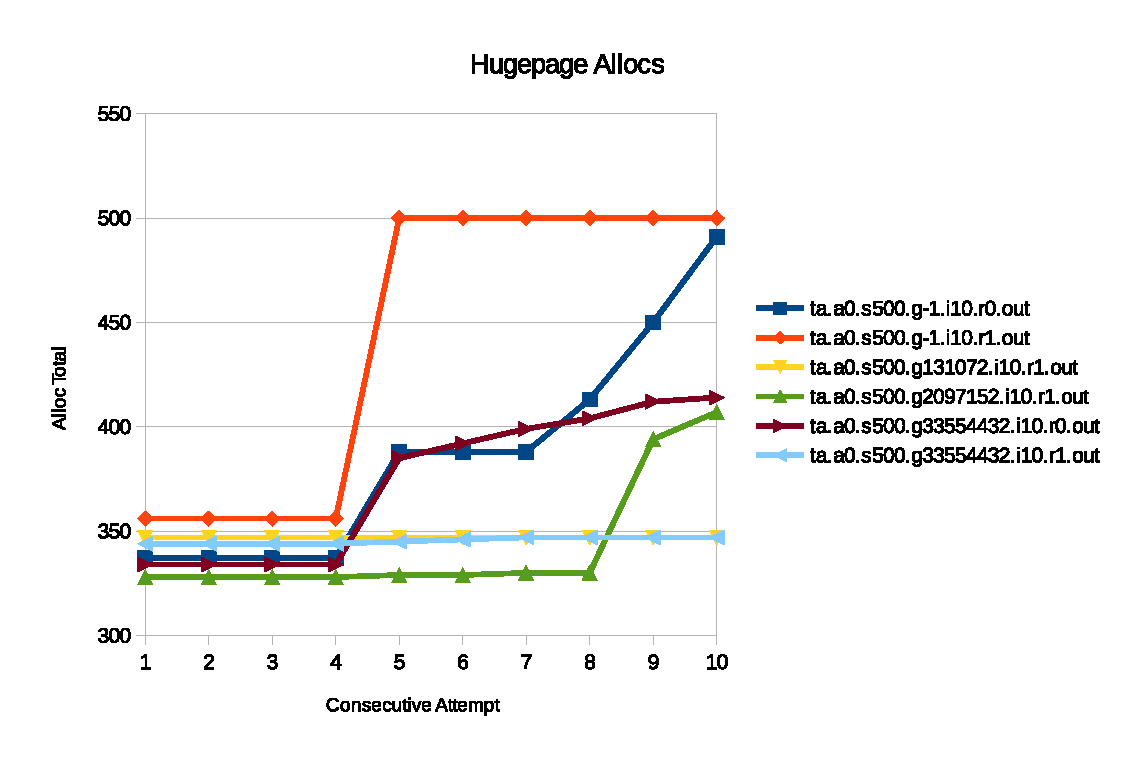
\includegraphics[width=\linewidth]{./datums/default_alloc.eps}
	\label{fig:default_alloc}
\end{figure}

As this chart shows, the default allocation strategy often struggles to fulfill a large huge page request at runtime. There are three key points on the graph to examine. The first is the initial allocation which for all attempts achieved roughly 350 pages of the 500 requested. The next key point is on consecutive attempt four, when 3 of the scenarios achieved a slightly higher allocation. The three in question are the two g-1s and the g33554432r0. Only the g-1r1 scenario achieves 500 at this point, and from thereafter the memory allocation succeeds, due to transparent hugepages keeping the pages available. The third key point is the 10th and final allocation attempt. At this juncture g-1r0 has almost, though not quite, fulfilled the 500 page request. g33554432r0 has slowly accumulated more pages but is only marginally greater than it was 6 attempts ago, and g2097152r1 has almost caught up with g33554432r0. Only the scenarios where no additional memory was taken by the test application actually achieved near 500 pages, and only two other allocations even achieved more than 350 pages allocated. When they did, it still took a large number of repeated requests to achieve only a small fraction more memory than the initial fulfillment. In order to demonstrate the efficacy of the proposed changes to the Linux kernel, we will now examine the proposed changes and then the data for the test scenarios.

\section{Wander}
There are two important changes to the alloc\_fresh\_huge\_page algorithm. First, if we completely fail to allocate any pages, we call try\_to\_free\_pages\footnote{http://lxr.free-electrons.com/source/mm/vmscan.c#L2826} (which frees up pages on that node which can be swapped out). Second, if we succeed in freeing pages then we re-attempt the allocation on that node. Additionally, we made a change to the calling algorithm, set\_max\_huge\_pages, where we will retry until either we succeed in fulfilling the allocation request or we fail at allocating any huge pages twice in a row.

\begin{figure}[H]
\lstinputlisting[firstnumber=1013, numbers=left, language=C, firstline=1013, lastline=1052]{../mm/hugetlb.c}
\label{figure:Aggressive alloc_fresh_huge_page}
\end{figure}

\begin{figure}[H]
\lstinputlisting[firstnumber=1643, numbers=left, language=C, firstline=1643, lastline=1665]{../mm/hugetlb.c}
\label{figure:Aggressive alloc_fresh_huge_page}
\end{figure}

The next chart shows the difference in success rates for this new strategy. The initial allocation is higher for all but one of the tests. This is a direct result, as shown by gathered statistics \footnote{see appendix C for gathered stats), of both the fault tolerance and retry changes we introduced.

\begin{figure}[H]
	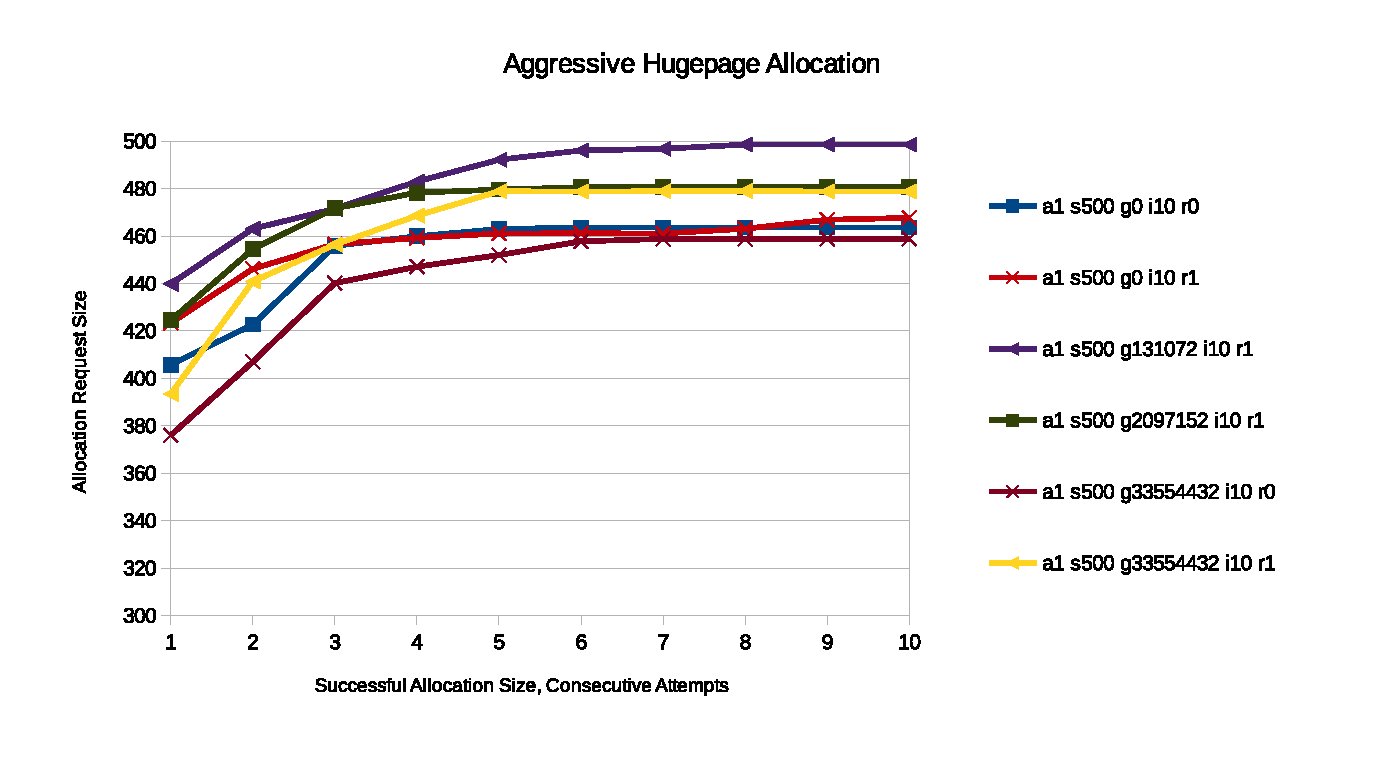
\includegraphics[width=\linewidth]{./datums/aggressive_alloc.eps}
	\label{fig:aggressive_alloc}
\end{figure}

\section{Postamble}
\section{Future Works}
\begin{appendices}
	\newpage
	\chapter{Appendix 1: Table}
		\section{Data Table}
		\begin{table}[h!]
			\caption{Hugepage Allocation Data Points}
			\label{table1}
				%some stuff goes here
			\end{table}
	\chapter{Appendix 2: List of Figures}
		\listoffigures
\end{appendices}
\end{document}